\justify
\section{Carreras tentativas comunes en los estudiantes de la UVG}

\justify
La s�ptima pregunta ten�a como prop�sito averiguar las carreras deseadas por los estudiantes durante la etapa tentativa. Estas se presentan en el siguiente cuadro.\\


\begin{table}[H]
	\begin{center}
		\caption{Categorizaci�n de carreras tentativas de los estudiantes encuestados ordenados por facultad.}
		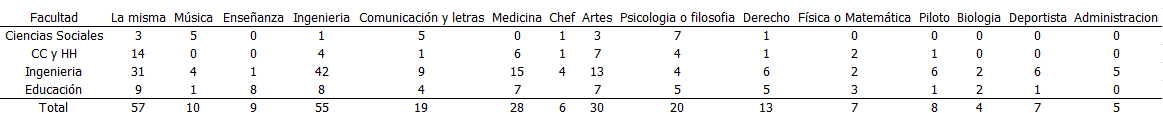
\includegraphics[scale=.50]{carreras-tentativas}
	\end{center}
\end{table}

Al analizar los datos obtenidos, se encuentra que aproximadamente un 80\% de los estudiantes tuvieron una carrera tentativa distinta a la carrera que estudian actualmente, y que solamente un 20\% sigui� la carrera deseada dentro de dicha etapa.\\

\begin{figure}[H]
	\begin{center}
		\caption{Comparaci�n entre los estudiantes que siguieron su carrera tentativa y los que no lo hicieron.}
		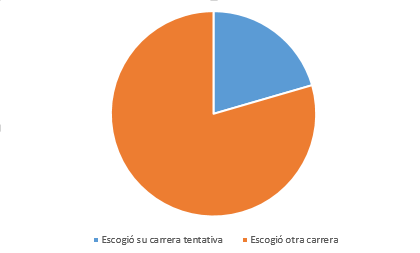
\includegraphics[scale=1]{propor-carrera-tenta}
	\end{center}
\end{figure}

Al analizar por facultad la gr�fica anterior (Cuadro O.2), se observa que en todas las facultades el porcentaje de estudiantes que no escogieron su carrera tentativa es mayor. Siendo la facultad de Ciencias y Humanidades la que tuvo el porcentaje m�s alto de estudiates que escogieron su carrera tentativa.\\

\begin{table}[H]
	\begin{center}
		\caption{Comparaci�n entre los estudiantes que siguieron su carrera tentativa y los que no lo hicieron por facultad.}
		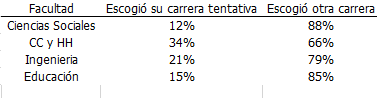
\includegraphics[scale=0.95]{cuadro-carrerast-facultad}
	\end{center}
\end{table}

En el cuadro O.3 se realiz� una estimaci�n de la proporci�n poblacional de los estudiantes de la Universidad del Valle de Guatemala que escogieron su carrera tentativa.\\

\begin{table}[H]
	\begin{center}
		\caption{Intervalo de confianza al 95\% de la proporci�n de los estudiantes que escogieron como carrera la carrera deseada en la etapa tentativa.}
		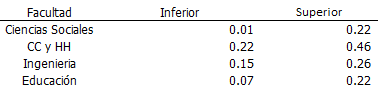
\includegraphics[scale=.95]{intervalo-confianza-carrerat}
	\end{center}
\end{table}

Con base en los cuadros anteriores, se puede decir que la proporci�n de estudiantes que actualmente estudian su carrera de etapa tentativa es menor, en todas las facultades, en comparaci�n con los que no la siguieron.\\